\clearpage
\section*{S25. Actual irregular Census blocks and contiguous missingness}
The reference domain contains 6,787 complete official 2020 Census blocks with P1 population 523,953. Within each complete block, GHSL weights are normalized before selecting the known-rate footprint. This avoids forcing every Census allocation unit into observed locations. The known-rate footprint retains 522,596.78 allocation units, 38,569 published DWR cells and 65,108 exact block--cell intersections. Originally missing rates and 1,333.22 allocation units outside this footprint remain outside the controlled reference; they are never assigned known hidden values.

The selected DWR mosaic item is the annual interval 1 October 2020--1 October 2021, distinct from the older multi-year footprint. We retrieve raw floating-point values with no palette/rendering transformation and convert the provider's feet to millimeters, divided by the exact interval duration in years. Rates are constant within published cells. Official NAD83 Census geometry and source-cell corners are projected to EPSG:3310 before exact intersections. Maximum polygon relative area-closure error is $2.31\times10^{-10}$; the conservative GHSL transfer has relative mass drift 0.000233, after which complete-block normalization fixes the Census total. The DWR footprint and rate layers share provider lineage; these are conditional method experiments, not independent geodetic truth.

With seed 20261001, each of 30 repetitions defines a random cell ordering and distances to one or four random spatial centres. The latter generate large contiguous holes on the irregular valid footprint. The same ordering nests 10, 30 and 50\% removals. The three thresholds are $-3$, $-5$ and $-10$ mm yr$^{-1}$. All 2,430 method--mask--threshold rows and nine unmasked baseline rows are retained.

Native observed-population prevalence extrapolates its measured class fraction to the block's originally known allocation. Area prevalence uses the observed area fraction. The unit-median rule classifies a whole block using the median of retained published-rate cells whose centres fall inside that block. No retained centre leaves the median rule undefined, even if a cell intersects the block. No retained population/area leaves the corresponding prevalence undefined. Undefined units are not assigned zero. In the unmasked baseline, the median rule already has 412 undefined blocks representing 4.386\% of known-footprint allocation. At $-5$ mm yr$^{-1}$, the native known class share is only 0.1308\%, so small errors must also be interpreted against this rare reference class.

We report both method-specific availability and signed/local-L1 errors on the intersection of computable blocks. Each repetition additionally retains method-specific conditional error and its exact denominator. On the entire originally known domain, class allocation is bounded by retained class mass and retained class mass plus all hidden allocation. Every known reference lies inside this accounting interval. Its width is hidden population allocation, not the removed pixel fraction, and is independent of the estimator. The numerical bound check is deterministic, not a confidence interval.
\begin{table}[htbp]\centering\small
\caption{Thirty-percent removal at the $-5$ mm yr$^{-1}$ cutoff: means over 30 fixed-mask repetitions. Unestimated share uses the known-footprint denominator; local L1 uses common-computable allocation. Bound width uses the whole known domain.}
\begin{tabular}{llrrr}\toprule
Mask & Method & Unestimated (\%) & Local L1 (pp) & Bound width (pp) \\\midrule
Random & Native prevalence & 0.20 & 0.00296 & 30.02 \\
Random & Area prevalence & 0.20 & 0.00608 & 30.02 \\
Random & Unit median & 9.41 & 0.01345 & 30.02 \\
One hole & Native prevalence & 23.01 & 0.00055 & 24.02 \\
One hole & Area prevalence & 23.01 & 0.00575 & 24.02 \\
One hole & Unit median & 26.80 & 0.01129 & 24.02 \\
Four holes & Native prevalence & 28.64 & 0.00197 & 30.97 \\
Four holes & Area prevalence & 28.64 & 0.00702 & 30.97 \\
Four holes & Unit median & 32.61 & 0.01332 & 30.97 \\
\bottomrule\end{tabular}
\end{table}
\begin{figure}[htbp]\centering
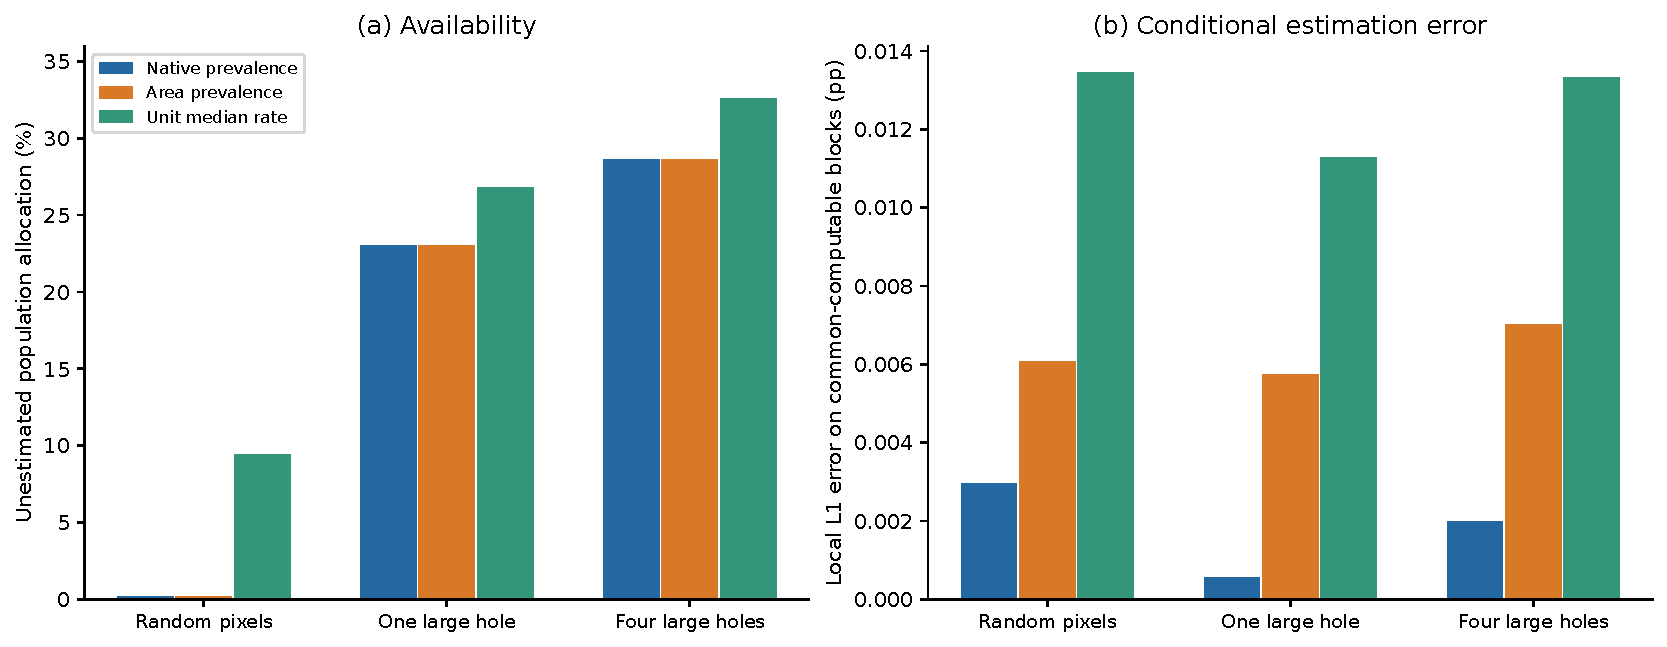
\includegraphics[width=\linewidth]{figures/additional_S25_real_blocks.pdf}
\caption{Availability and conditional estimation error on actual irregular Census blocks. Bars are repetition means for 30\% removal and the $-5$ mm yr$^{-1}$ cutoff. Each estimator uses identical missingness; the right panel omits noncomputable blocks by definition. Small local error must therefore be read alongside the left-panel unidentified mass. Full 10/30/50\% and threshold results are supplied in the CSV archive.}\label{fig:addreal}
\end{figure}

At 30\% removal, native prevalence's unestimated allocation ranges from 0.064--0.307\% for random pixels, 3.73--44.98\% for one hole and 14.82--47.99\% for four holes. Mean class bounds are [0.0903,30.1064], [0.0859,24.1010] and [0.0977,31.0655]\%, respectively. Neither low conditional L1 error nor random-mask performance supports assigning a class to entire genuinely missing blocks. Full replicates, per-method denominators, bounds and source hashes are in \path{additional/real_block_masking/}.
\clearpage
\section*{S26. Buffered spatial recalibration and shared-acquisition influence}
This exploratory analysis checks how conclusions change when calibration and dependence are treated more strictly. It does not retrain GHSL or WorldPop, validate individual households or supply a probability interval for unknown interferograms.

For the same 319 complete Fresno block groups as S24, projected polygon-centroid ranks define five west--east or south--north spatial bands. One band is held out at a time. At 0 m, all other groups train the total multiplier. At 1 or 3 km, training polygons touching or within that distance of the held-out polygon union are excluded. Every retained training set has at least 30 groups, and every held-out group is predicted exactly once per design. Calibration factors use training ACS totals only. Model values and geometry remain fixed. We retain 90 fold--model records, every group assignment and 18 full-domain held-out summaries. The 80 ACS variance replicates quantify the survey component of signed fold-total error, conditional on the fixed population grids; they are not population-model error or evidence of source independence.
\begin{table}[htbp]\centering\small
\caption{Spatial recalibration against ACS. Ranges span two spatial axes and three buffers, not independent replicates or confidence intervals.}
\begin{tabular}{lrrrr}\toprule
Released grid & Raw WAPE (\%) & In-sample (\%) & Held-out WAPE (\%) & Held-out total error (\%) \\\midrule
GHSL & 34.89 & 33.16 & 33.24--33.85 & -0.03--+3.64 \\
WorldPop & 33.22 & 32.29 & 32.34--32.98 & -0.04--+3.78 \\
Census\_2020\_P1 & 19.93 & 19.93 & 19.94--20.07 & -0.27--+0.58 \\
\bottomrule\end{tabular}
\end{table}

The in-sample total match cannot be interpreted as out-of-area validation. Held-out GHSL and WorldPop WAPE remains above 32\%, and the 3-km west--east design has signed total errors of +3.64 and +3.78\%, respectively, compared with +1.39 and +1.43\% for the south--north design. Calibration is imperfectly transferable even within this one domain.

For sampling, each of the 225 dates in the 224-pair pool is deleted with all incident edges, not one edge at a time. We recompute summaries under equal-pair weights and under equal weights for the retained 28 year--quarter strata. All strata survive each deletion. The maximum deletion removes seven pairs. The retained graph has 28--34 components, compared with 29 at baseline, and remains separate from the connected 437-pair processing stack. For $q=0.3$ population weighting, the equal-quarter change spans $-0.3856$ to $+0.1647$ pp. Full results cover four support definitions and three allocation weightings (2,700 date--support--weight rows).

This is a delete-date influence diagnostic for fixed observed support values. It neither re-solves the velocity inversion nor treats the disconnected support pool as a processing network. Because shared reference, atmospheric structure and acquisition effects remain dependent, we do not form an iid jackknife confidence interval. Source hashes and graph/stratum checks accompany the fold and deletion tables in \path{additional/spatial_acquisition/}.
\begin{figure}[htbp]\centering
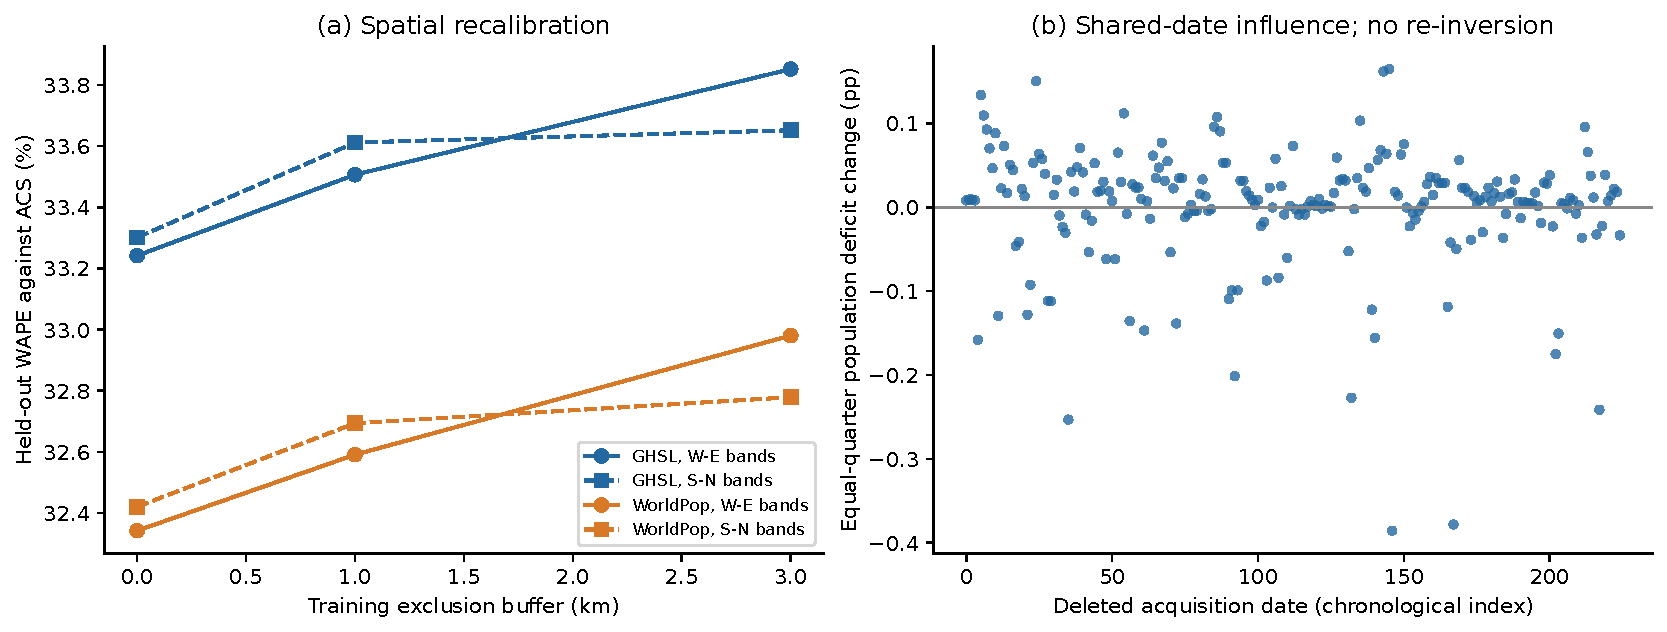
\includegraphics[width=\linewidth]{figures/additional_S26_dependence.pdf}
\caption{Spatially held-out recalibration and shared-date influence. Left: training-only calibration under two five-band partitions and three exclusion buffers. Right: population-weighted $q=0.3$ equal-quarter change after deleting every edge incident to one date. Each point is a dependent sensitivity case; no confidence interval or velocity re-inversion is implied.}\label{fig:adddependence}
\end{figure}
\clearpage
\section*{S27. Training-only quality rules and coverage--residual curves}
We freeze 18 rules before reading their coverage/error curve: finite training velocity; the original training mask; training mean-coherence cutoffs 0.05/0.2/0.3/0.4/0.5/0.6/0.7; training residual RMS limits 0.5/1/1.5/2 mm; and training velocity-standard-deviation limits 0.5/1/2/5/100 mm yr$^{-1}$. Every metric and the reference region are obtained from training pairs only. Rules are post-filters on one fixed training inversion, not repeated inversion fits. No rule is chosen to minimize held-out error.

All 44 excluded unwrapped edges are reconstructed from the retained training time series using their actual dates, the training reference region and the Sentinel-1 phase-to-LOS coefficient. Training and excluded edge sets are disjoint; acquisition dates need not be. Raw recomputation reproduces the frozen S7 finite-velocity pool to a maximum pixel-RMSE difference of $1.69\times10^{-7}$ mm. Each quality rule reports accepted full-domain area/population coverage, evaluable accepted coverage, allocation lacking an excluded-edge residual, pooled pixel--edge RMSE, population-weighted pooled RMSE, pixel median/P95 and per-edge ranges. Accepted and evaluable population coverage coincide here; that equality is checked rather than assumed.
\begin{table}[htbp]\centering\small
\caption{Selected training-only rules. Coverage denominator is the complete matched ROI. Residual units are LOS displacement millimeters; velocity-standard-deviation cutoffs are mm yr$^{-1}$. All 18 rules and all 44 edge rows per rule remain in the archive.}
\begin{tabular}{lrrrr}\toprule
Rule & Population (\%) & Area (\%) & Pooled RMSE (mm) & Population RMSE (mm) \\\midrule
Finite velocity & 100.00 & 99.99 & 0.984 & 0.359 \\
Training mask & 99.86 & 97.49 & 0.699 & 0.350 \\
$q\geq0.2$ & 99.40 & 87.62 & 0.491 & 0.344 \\
$q\geq0.3$ & 98.27 & 80.49 & 0.429 & 0.340 \\
$q\geq0.4$ & 95.34 & 71.69 & 0.388 & 0.336 \\
$q\geq0.7$ & 41.04 & 23.65 & 0.331 & 0.317 \\
$\sigma_v\leq0.5$ & 4.17 & 4.11 & 0.317 & 0.288 \\
$\sigma_v\leq1$ & 31.16 & 25.55 & 0.377 & 0.360 \\
\bottomrule\end{tabular}
\end{table}
\begin{figure}[htbp]\centering
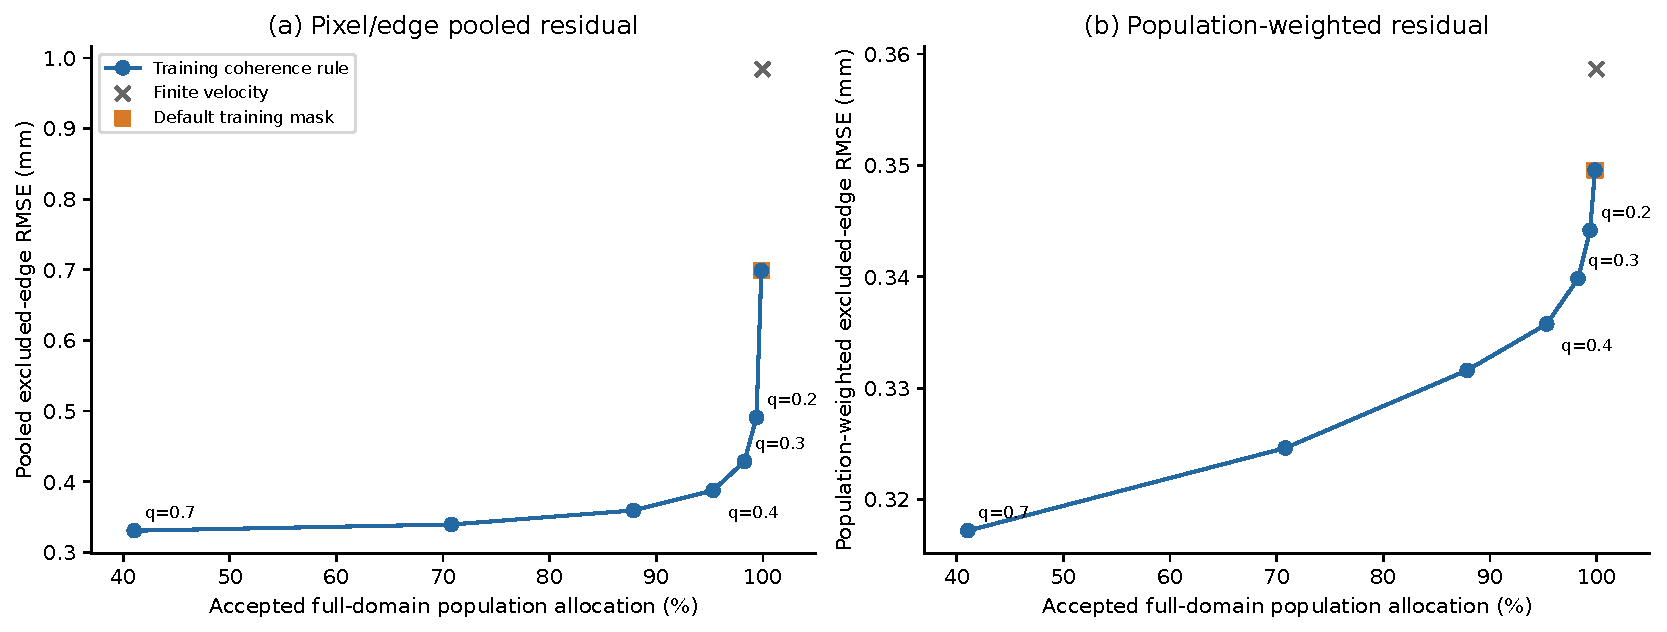
\includegraphics[width=\linewidth]{figures/additional_S27_quality_curve.pdf}
\caption{Coverage--residual curve under training-only coherence filtering. Points use the original training mask plus the stated coherence rule; finite velocity and default training-mask baselines are also shown. The right panel weights residual observations by population allocation. Connections guide the eye and do not imply independent points or optimization.}\label{fig:addquality}
\end{figure}

Tightening coherence improves internal residuals here while reducing accepted allocation. Other training metrics need not order the population-weighted error monotonically: the 0.5 and 1 mm yr$^{-1}$ velocity-standard-deviation filters give population-weighted RMSE 0.288 and 0.360 mm while admitting 4.17 and 31.16\% of population allocation. Both filter outcomes are retained. Shared acquisitions, reference and atmospheric signals prevent interpreting these residuals as external velocity accuracy. Invalid or unobserved locations are not validated by a filter. Full source provenance, 18-rule summary and 792 rule--edge rows are in \path{additional/training_quality/}.
\clearpage
\section*{S28. Two fixed additional regions using archived ARIA products}
The new-region protocol is fixed before their allocation outcomes: Los Angeles [$-118.4$,$-118.1$]$^\circ$ E by [33.85,34.10]$^\circ$ N and Davis--Sacramento [$-121.9$,$-121.6$]$^\circ$ E by [38.4,38.7]$^\circ$ N. We use GHSL R2023A 2020 population at 3 arcsec and the April 2026 archived ARIA California products of Sangha et al.\ \citep{sangha2026california,sangha2026data}. Los Angeles uses ascending track A064 (reference P597); Davis--Sacramento uses A137 (P266). Completed notebook outputs and the published track table document periods 14 February 2016--13 May 2022 and 3 March 2017--29 August 2023. Some archived A137 run notes/configurations give older dates; that conflicting metadata is preserved rather than silently treated as authoritative. The GeoTIFF tags alone do not certify a temporal model.

Support here means finite, nonzero published LOS velocity together with mean spatial coherence at least 0.2, 0.3 or 0.4. The zero exclusion follows the provider notebook. This differs from individual-pair unwrapped/coherence support and from a final LiCSBAS mask; identical cutoff values do not make these support definitions equivalent. No physical rate threshold is used for the population-support comparison.

We intersect the published raster support with GHSL source pixels and the fixed rectangles using spherical latitude/longitude area fractions, preserving extensive counts. Integration produces a support fraction for each clipped native GHSL cell; that fraction is held constant within that cell for subsequent reporting-grid comparisons. Thus the larger-scale exact partition applies to this declared piecewise-constant integrated field, not to a household-level support map. The fixed totals are 3,638,746.86 allocation units for Los Angeles and 167,055.45 for Davis--Sacramento. Every 250/500/1,000/2,000-m grid and zero/half-cell origin conserves that total. Signed allocation differences, local L1, Cauchy bounds and top-decile allocation-deficit overlap are retained for all 96 designs. Bounds are checked per reporting cell; relative closure tolerances are below $10^{-9}$. Ranking overlap is not a measurement-priority or physical-risk validation.
\begin{table}[htbp]\centering\small
\caption{Uniform-minus-native allocation differences (pp of fixed population total) across all four scales and four origins per cutoff. Small and identical-threshold cases remain in the results.}
\begin{tabular}{lrrr}\toprule
Region & Coherence cutoff & Minimum (pp) & Maximum (pp) \\\midrule
Los Angeles & 0.2 & 0.0255 & 0.1567 \\
Los Angeles & 0.3 & 0.0255 & 0.1567 \\
Los Angeles & 0.4 & 0.0257 & 0.1859 \\
Davis--Sacramento & 0.2 & 0.0511 & 0.3723 \\
Davis--Sacramento & 0.3 & 0.0511 & 0.3723 \\
Davis--Sacramento & 0.4 & 0.0511 & 0.3723 \\
\bottomrule\end{tabular}
\end{table}
\begin{figure}[htbp]\centering
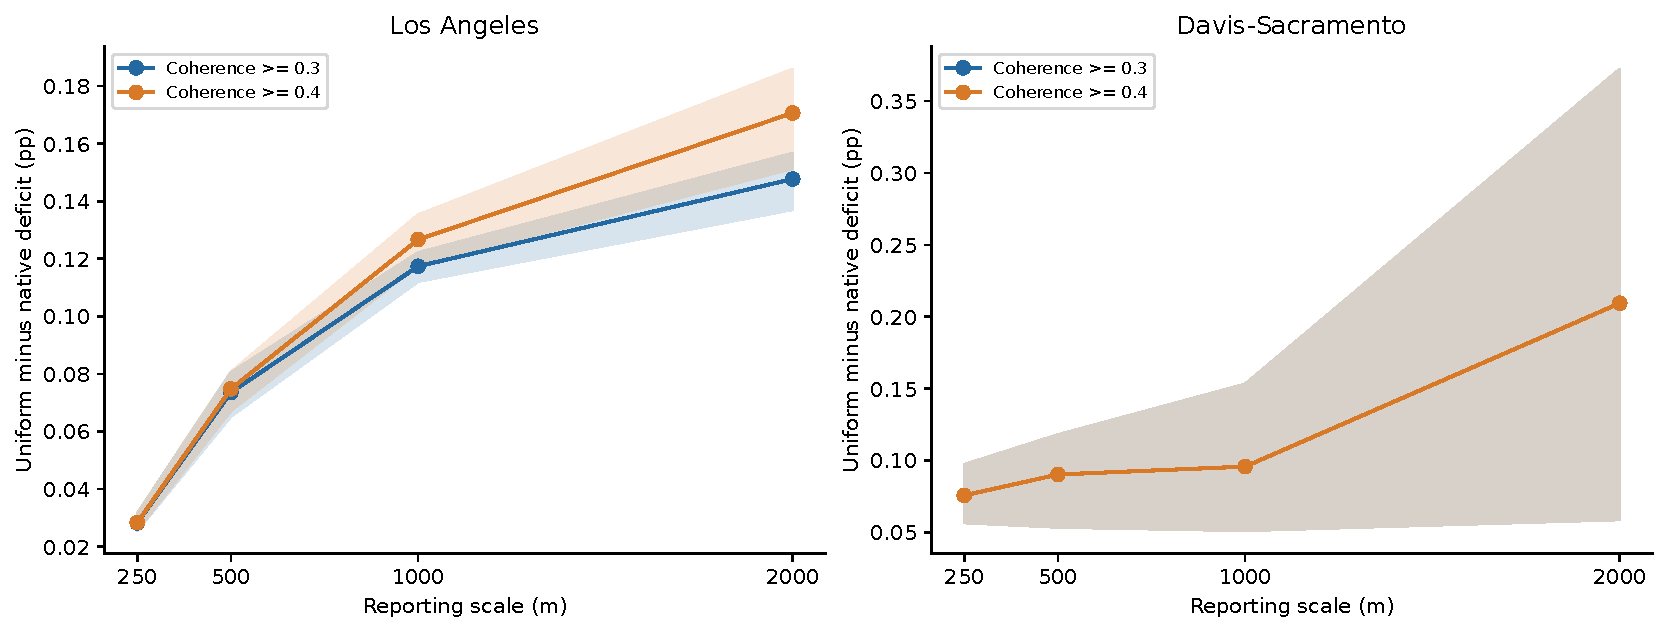
\includegraphics[width=\linewidth]{figures/additional_S28_new_regions.pdf}
\caption{Allocation effects in the two fixed additional regions. Lines are means across four origins; bands span those origins and are not confidence intervals. Cutoffs 0.3 and 0.4 coincide in Davis--Sacramento and partly overlap in Los Angeles. These much smaller effects prevent generalizing the primary-case magnitude.}\label{fig:addregions}
\end{figure}
\clearpage
\section*{S29. Municipal residential eligibility as a distinct ancillary reference}
The public City of Fresno Existing Land Use layer (hosted FeatureServer layer 19) supplies a classification source distinct from the satellite built-surface layer \citep{fresno2026landuse}. We obtain all 123,493 features intersecting the fixed rectangle, check unique ObjectIDs and retain only ObjectID, ELU, ELUText and LayerRefreshDate. No owner or address fields are collected. Strict residential codes are rl/rml/rm/rmh/rh/rr/rmht/run; the broader rule additionally admits raur/rmx/cmx/cce mixed-use or agricultural-residential classes. Both semantic rules are frozen before the allocation comparison. Unclassified and unmapped locations remain unknown; they are not assigned nonresidential status. The source metadata and refresh dates do not establish a 2020 land-use vintage.

Within complete Census blocks and the common projected 100-m population grid of S20, we intersect municipal geometry with each block--cell piece in EPSG:3310. Seventeen invalid polygons are repaired using make\_valid; overlapping class fragments are unioned before measuring area, separately for mapped, strict and broader eligibility. All 88,865 pieces satisfy nested eligibility fractions and the [0,1] bounds. Population remains uniform within its source cell. DWR footprint fraction is also the spatially averaged value in each projected 100-m cell; no house-level radar support is inferred.

We first diagnose where the unrestricted block-normalized population falls: residential eligibility, mapped other land use, or unmapped classification. Strict residential eligibility contains 85.22\% of mapped GHSL allocation and 89.30\% of mapped CA-POP allocation, but unmapped classification represents 32.22 and 31.26\% of their complete denominators. The broader definition gives 85.29 and 89.38\% within mapped allocation. These agreement fractions are not independent resident counts. Other land-use allocation may reflect mixed use, group quarters, source-cell mixing, classification error or vintage mismatch; it is not automatically false population.

For allocation sensitivity, each rule is normalized to the same complete-block Census count before support summaries are formed. Area-uniform, GHSL, CA-POP, municipal residential-area uniform and GHSL/CA-POP restricted to eligibility are compared on a joint domain where all six have a positive denominator. The strict domain retains 4,879 blocks and 466,999 Census allocation units (89.13\% of the complete total); the broader domain retains 4,885 blocks and 467,490 units (89.22\%). Both fail the initial 90\% diagnostic coverage gate. We retain that failure explicitly and report the limited common-domain diagnostic, rather than extrapolating it to full Fresno. Excluded masses are 56,954 and 56,463, respectively.
\begin{table}[htbp]\centering\small
\caption{Support deficit on the joint common Census-allocation domain. Each row conserves the same block total within each definition; the strict and broader domains differ and cover only 89.13--89.22\% of the complete population.}
\begin{tabular}{lrr}\toprule
Allocation rule & Strict deficit (\%) & Broader deficit (\%) \\\midrule
Area uniform & 0.21931 & 0.21908 \\
GHSL & 0.09267 & 0.09257 \\
CA-POP & 0.05721 & 0.05715 \\
Residential area & 0.08886 & 0.08877 \\
GHSL restricted & 0.05076 & 0.05071 \\
CA-POP restricted & 0.04136 & 0.04132 \\
\bottomrule\end{tabular}
\end{table}
\begin{figure}[htbp]\centering
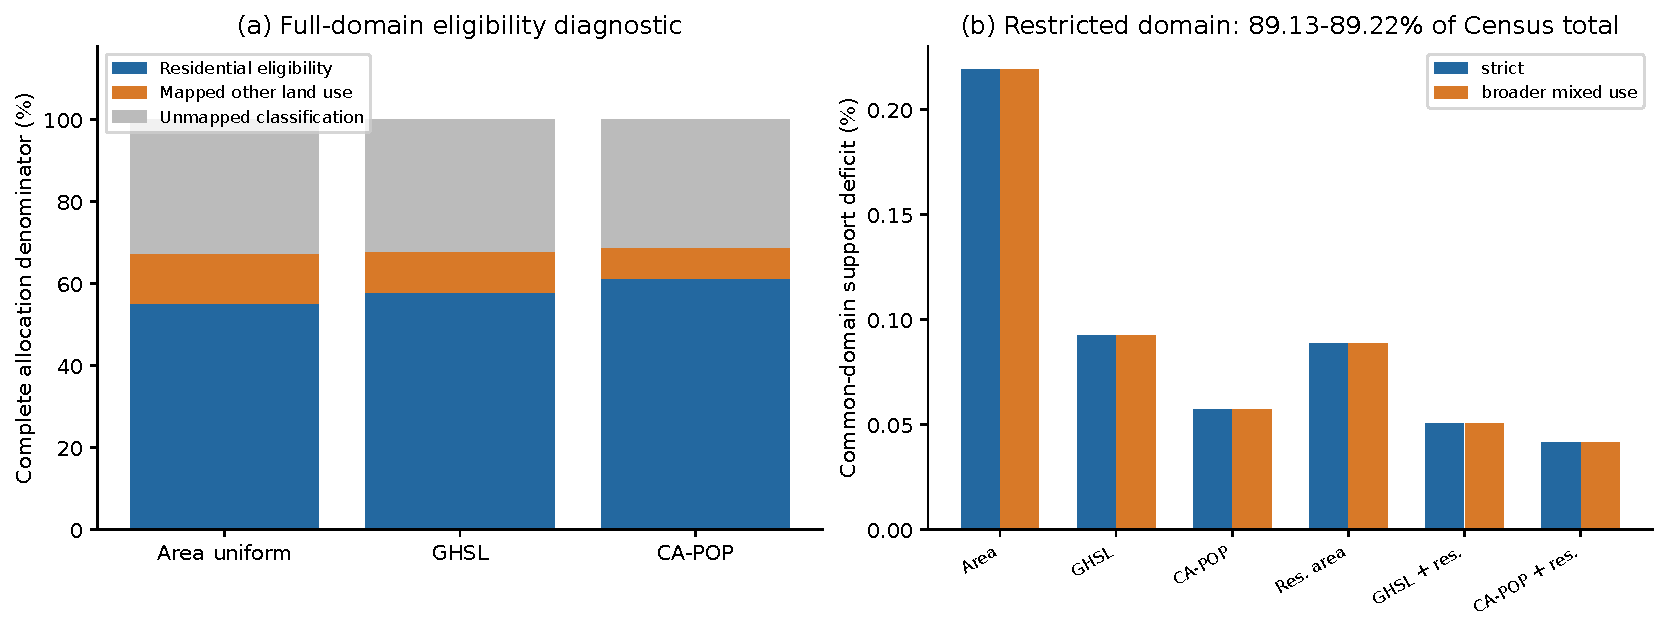
\includegraphics[width=\linewidth]{figures/additional_S29_residential.pdf}
\caption{Municipal land-use eligibility and allocation sensitivity. Left: all complete allocation units partitioned into residential, mapped other use and unmapped classification. Right: six rules on their restricted common domain. The unmapped category and failed initial 90\% diagnostic gate are retained; neither a residential restriction nor a smaller deficit establishes improved household truth.}\label{fig:addresidential}
\end{figure}

The added reference strengthens source diversity at the eligibility level only. It does not establish independence of Census-based population counts, remove the CA-POP/GHSL allocation assumptions or validate deformation in gaps. All feature metadata, category choices, geometry diagnostics, per-block allocations and source hashes are archived in \path{additional/residential_allocation/} and the selected-source companion.
\clearpage
\section*{S30. Archived independent GNSS transfer with disjoint frame controls}
We use independent NGL GNSS observations already projected into the LOS geometry and track periods in the completed Sangha et al.\ notebooks \citep{sangha2026california,sangha2026data}. Their station screening is retained, including the provider completeness and residual-scatter criteria; no station is selected using our comparison residual. Notebook cell 38 reports 411 A064 and 341 A137 LOS rates, explicitly converted from m yr$^{-1}$ to mm yr$^{-1}$. We join station names to the public NGL coordinate metadata downloaded on 1 October 2026 \citep{ngl2026holdings}. The fixed rectangles contain 12 and five eligible archived stations. The provider reference P597/P266 lies outside the respective rectangle but is retained as a frame control.

Before reading residuals, station coordinates alone select the eligible site closest to each rectangle's centre as an alternative local control: MHMS and UCD1. Provider reference and local-control stations are excluded from every validation metric, including metrics using the other control. Thus the same 11 Los Angeles and four Davis--Sacramento validation stations are compared under both frames. For each control $r$, both products use the relative quantity $v_i-v_r$; no regression or spatial ramp is fitted to validation stations. The nearest-centre choice is an exploratory local-frame sensitivity, not an externally validated optimal reference.

Native samples use the containing cell, calculated with floor through rasterio.index, not rounded pixel-corner indices. Sensitivities use the median within one- and three-pixel-radius windows. Published zero exclusions are preserved except at the provider reference itself. All 19 selected site windows are losslessly archived as 7-by-7 float32 source capsules, together with the complete source-raster hashes, row/column indices and centre coordinates; the full GeoTIFFs are also supplied in the source companion. Reproduction from capsules gives the same station and summary tables as the complete rasters. Maximum station-to-containing-pixel-centre offsets are 57.96 and 40.10 m. All sites and every unavailable sample are recorded; none is removed for a large residual.

The exact archived MintPy implementation confirms that get\_los\_obs with an omitted model argument invokes a polynomial degree-1 fit, without periodic or earthquake-step terms. The published InSAR trend uses additional seasonal/step terms. Although periods and spatial frames follow the completed notebooks, the temporal models are therefore not identical. The April data release also retains conflicting older A137 configuration dates. These are source-version and trend-comparison limitations, not presumed corrections. We have not newly refitted raw daily GNSS or silently resolved the conflicts using the best-looking residual.
\begin{table}[htbp]\centering\small
\caption{Relative LOS comparison with archived independent GNSS observations. Bias is at the containing native pixel; RMSE columns give pixel radii 0, 1 and 3. All units are mm yr$^{-1}$. Controls are excluded from every metric.}
\begin{tabular}{llrrrrr}\toprule
Region & Control & $n$ & Bias & RMSE 0 & RMSE 1 & RMSE 3 \\\midrule
Los Angeles & P597 & 11 & -14.43 & 14.49 & 14.43 & 14.34 \\
Los Angeles & MHMS & 11 & +0.01 & 1.30 & 1.32 & 1.38 \\
Davis--Sacramento & P266 & 4 & +6.68 & 8.94 & 9.08 & 8.98 \\
Davis--Sacramento & UCD1 & 4 & +9.07 & 10.85 & 11.16 & 11.21 \\
\bottomrule\end{tabular}
\end{table}
\begin{figure}[htbp]\centering
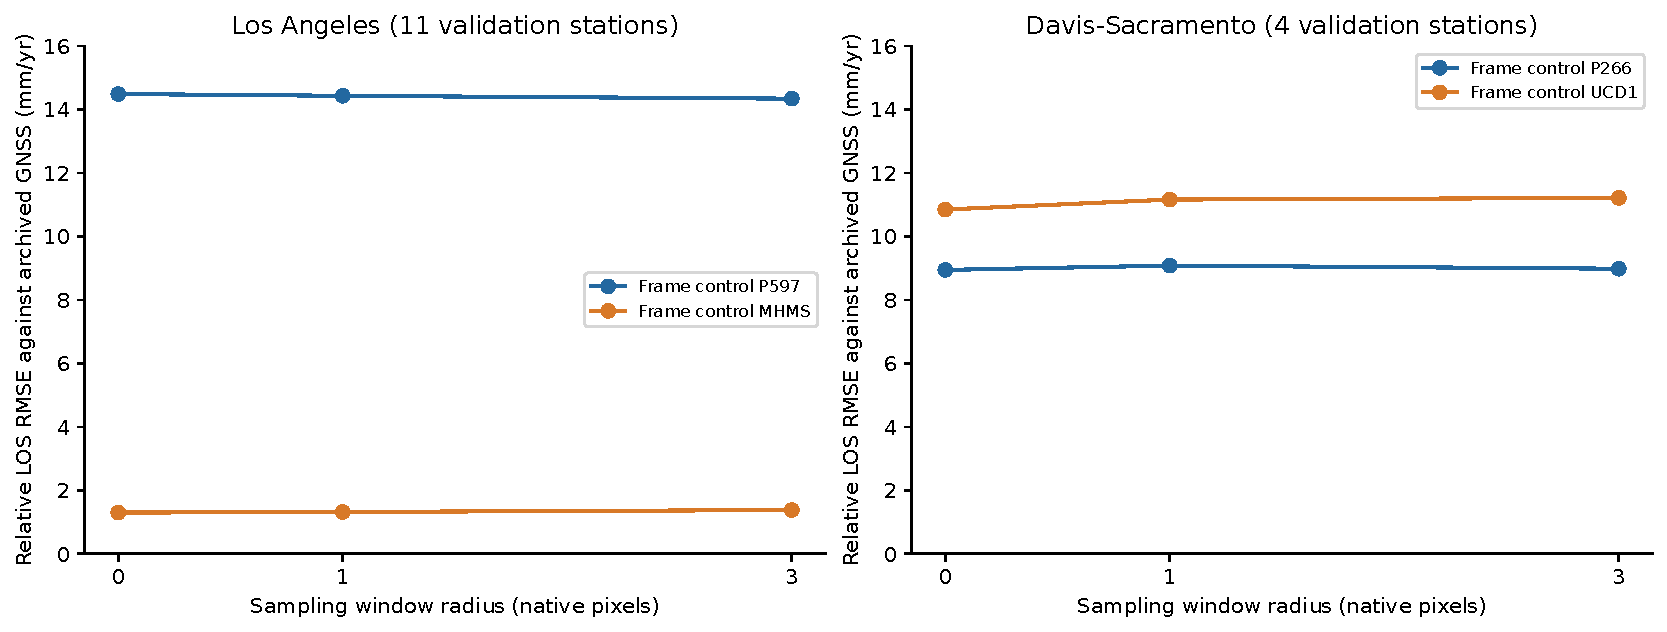
\includegraphics[width=\linewidth]{figures/additional_S30_GNSS.pdf}
\caption{External LOS/GNSS consistency under two disjoint frame controls and three sampling radii. The same validation sites are used within each region. Los Angeles improves under the local frame, while Davis--Sacramento does not. The entire result is retained; the favorable Los Angeles value cannot be generalized to the second region or to Bangkok.}\label{fig:addgnss}
\end{figure}

FGNW and FGSW are within 100 m and are assigned one collocation cluster. Los Angeles therefore has 11 validation stations but ten descriptive clusters; Davis--Sacramento has four and four. At radius 0 with local controls, cluster-median RMSE is 1.20 and 10.85 mm yr$^{-1}$. Shared frame-control error, nearby monuments and spatial signals prevent treating station errors as independent trials; no iid confidence interval is reported. Radar scattering targets and GNSS monuments may also measure different local motion.

This comparison introduces independent observations for an archived external California LOS product and tests sensitivity to spatial reference. It does not independently validate our Bangkok inversion, household placement, support masks or genuinely missing rates. The large Davis--Sacramento discrepancies and temporal-model conflicts remain unresolved evidence limits, so we do not call the exercise a successful physical validation. Station-level estimates, all frame/radius summaries, exclusions, collocation assignments, source notebooks and implementation excerpts are retained in \path{additional/gnss_transfer/} and the source companion.
